\documentclass[12pt]{amsart}
\usepackage{amsaddr}
\usepackage{marktext} 
%% Remove draft for real article, put twocolumn for two columns
\usepackage{svmacro}
\usepackage[utf8]{inputenc}
\usepackage{enumitem}
\usepackage[style=alphabetic, backend=biber]{biblatex}
\addbibresource{bibliography.bib}

%% commentary bubble
\newcommand{\SV}[2][]{\sidenote[colback=green!10]{\textbf{SV\xspace #1:} #2}}

%% Title 
\title{ MATH 102: MIDTERM }
\author{Name:\_\_\_\_\_\_\_\_\_\_\_\_\_\_\_\_\_\_\_\_ ID: \_  \_  \_   \_  \_  \_  \_  \_ 
\\   Good Luck!}

%\author{Co-author}
%\address{  }
%\email {  }
%
\date{Oct 12, 2023}

\begin{document}

\maketitle


There are five questions. Make sure you justify all your work for complete credit.

\section*{Rules}

\begin{itemize}[leftmargin=*]
	\item You have 80  minutes to complete your work..
	\item Closed books.
	\item No use of internet, textbooks, computer algebra systems, calculators.
	\item No collaboration.
	\item 1 person per bathroom break. When you go to the bathroom, turn in your cellphone and exam until return.
\end{itemize}

\newpage

\section*{Questions}

\begin{enumerate}[label=\arabic*.,itemsep=10pt, leftmargin=*]
	\item\textit{[20 points.]}
	\begin{enumerate}
		\item \textit{[10 points.]}
		      Can you fill the following chessboard with 2x1 domino pieces? Explain your answer.
		      \begin{center}
			      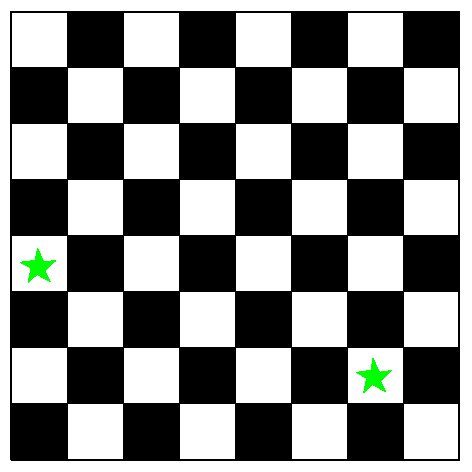
\includegraphics[width=0.5\textwidth]{Checker1.pdf}
		      \end{center}
		      \vspace{5cm}

		\item \textit{[10 points.]}
		      Show that the square of an odd integer is again odd by direct proof
		      from definition.


	\end{enumerate}
	\newpage
	\item\textit{[20 points.]}
	The symmetric difference of two sets $A$ and $B$ is defined as follows
	\begin{equation*}
		A \triangle B = (A\setminus B) \cup (B\setminus A) \,.
	\end{equation*}
	\begin{enumerate}
		\item \textit{[10 points.]}
		      Use the Venn diagram to represent $A \triangle B$.
		\item \textit{[10 points.]}
		      Let $A = \set{1,2,3,4,5,6,7}$ and $B = \set{2,4,6}$. What is $A\triangle B$?
	\end{enumerate}
	\newpage


	\item\textit{[20 points.]}
	What is Bezout's identity? Give 2 examples.

	\newpage

	\item \textit{[20 points.]} Prove that if $a \mid bc$ and $\gcd(a,b) = 1$, then $a \mid c$.

	      \newpage

	\item \textit{[20 points.]} For any sets $A$ and $B$, prove that
	      \begin{equation*}
		      A \triangle B \subseteq A \cup B \,.
	      \end{equation*}
	      Hint: Start with ``Let $x$...'' and use definitions of the operations.

\end{enumerate}



\printbibliography
%\bibliography{refs}
%\bibliographystyle{halpha-abbrv}


\end{document}
